 \chapter{Line Integrals}%endchapter 
 \label{chapter:line}
 
  So far we have always insisted all curves and parametrizations are differentiable or $C^1$.
  We now relax this requirement and subsequently only assume that  all curves (and parametrizations) are \negrito{piecewise differentiable}, or \negrito{piecewise $C^1$}.
  \begin{definition}
    A function $f:[a, b] \to \bbR^n$ is called \negrito{piecewise $C^1$} if there exists a finite set $F \subseteq [a, b]$ such that $f$ is $C^1$ on $[a, b] -F$, and further both left and right limits of $f$ and $f'$ exist at all points in $F$.
  \end{definition}


  
  
  \begin{figure}[h]
  \centering
  \scalebox{0.8}{
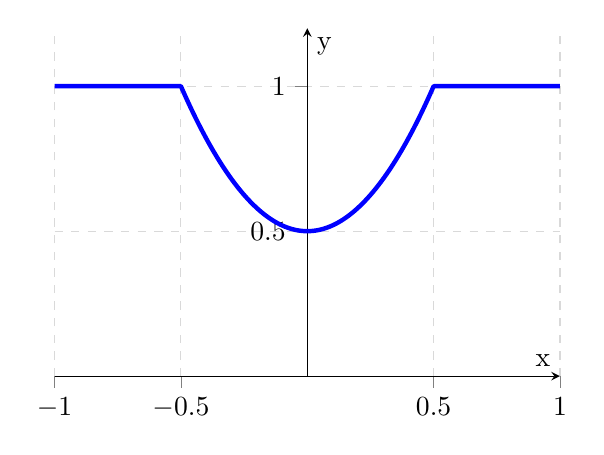
\begin{tikzpicture}
    \begin{axis}[
        axis x line=middle,
        axis y line=middle,
        grid = major,
        width=8cm,
        height=6cm,
        grid style={dashed, gray!30},
        xmin=-1,     % start the diagram at this x-coordinate
        xmax= 1,    % end   the diagram at this x-coordinate
        ymin= 0,     % start the diagram at this y-coordinate
        ymax= 1.2,   % end   the diagram at this y-coordinate
        xlabel=x,
        ylabel=y,
		/pgfplots/xtick={-1, -0.5, ..., 1}, % make steps of length 0.5
		/pgfplots/ytick={0, 0.5, ..., 1}, % make steps of length 0.5
        tick align=outside,
        enlargelimits=false]
      % plot the function
	  \addplot[domain=-1:1, blue, ultra thick,samples=500] {x < -0.5 ? 1 : (x < 0.5 ? x^2/0.5 +0.5 : 1)};
    \end{axis}
\end{tikzpicture}} 
\caption{Piecewise $C^1$ function}
  \end{figure}

    \begin{definition}
    A (connected) curve $\caminho$ is \negrito{piecewise $C^1$} if it has a parametrization which is continuous \emph{and} piecewise $C^1$.
  \end{definition}
  
   \begin{figure}[h!]
  \begin{center}
  \begin{tikzpicture}
   \draw (0,0) -- (3,0) -- (3,3) -- (0,3) -- (0,0);
  \end{tikzpicture}
  \end{center}
  \caption{The boundary of a square is a piecewise $C^1$ curve, but not a differentiable curve.}
    \end{figure}

  \begin{remark}
    A piecewise $C^1$ function need not be continuous.
    But curves are always assumed to be at least continuous; so for notational convenience, we define a piecewise $C^1$ curve to be one which has a parametrization which is both continuous and piecewise $C^1$.
  \end{remark}
  
 


 
 
  \section{Line Integrals of Vector Fields}
  We start with some motivation.  With this objective we remember the definition of the work:

  \begin{definition}
    If a constant force $\funvect{f}$ acting on a body produces an  displacement $\Delta\vector{ x}$, then the \negrito{work} done by the force is $\funvect{f} \bp \Delta \vector{ x} $.
  \end{definition}
  
We want to generalize this definition to the case in which the force is not constant.  For this purpose let $\caminho \subseteq \bbR^3$ be a curve, with a given direction of traversal, and $\funvect{f}:\bbR^3 \to \bbR^3$ be a vector function.

  Here $\funvect{f}$ represents the force that acts on a body and pushes it along the curve $\caminho$.
  The work done by the force can be approximated by
  \begin{equation*}
    W \approx \sum_{i = 0}^{N-1} \funvect{f}( x_i ) \bp ( \vector{x}_{i+1} -  
\vector{x}_i ) =\sum_{i = 0}^{N-1} \funvect{f}( x_i ) \bp  \Delta\vector{x}_i
  \end{equation*}
  where $ \vector{x}_0$, $ \vector{x}_1$, \dots, $ \vector{x}_{N-1}$ are $N$ 
points on $\caminho$, \emph{chosen along the direction of traversal}.
  The limit as the largest distance between neighbors approaches $0$  is the work done:
  \begin{equation*}
    W = \lim_{\norm{P} \to 0} \sum_{i = 0}^{N-1} \funvect{f}( x_i ) \bp  \Delta\vector{x}_i
  \end{equation*}
  

 This motivates the following definition:
  
  \begin{definition}
    Let $\caminho \subseteq \bbR^n$ be a curve with a given direction of traversal, and $\funvect{f}:\caminho \to \bbR^n$ be a (vector) function.
    The \negrito{line integral} of $\funvect{f}$ over $\caminho$ is defined to be
    \begin{align*}
      \dint_\caminho \funvect{f} \bp \dif \ell &= \lim_{\norm{P} \to 0}
	\sum_{i = 0}^{N-1} \funvect{f}(  \vector{x}_i^* ) \bp (  \vector{x}_{i+1} 
-  \vector{x}_i )\\
&=\lim_{\norm{P} \to 0}
	\sum_{i = 0}^{N-1} \funvect{f}(  \vector{x}_i^* ) \bp \Delta\vector{x}_i .
    \end{align*}
    Here $P = \set{ \vector{x}_0,  \vector{x}_1, \dots,  \vector{x}_{N-1}}$, 
the points $x_i$ are chosen along the direction of traversal, and $\norm{P} = 
\max \abs{ \vector{x}_{i+1} -  \vector{x}_i}$.
  \end{definition}
  
  
 


  

  \begin{remark}
    If $\funvect{f} = (f_1, \dots, f_n)$, where $f_i:\caminho \to \bbR$ are functions, then one often writes the line integral in the \negrito{differential form} notation as
    \begin{equation*}
      \dint_\caminho \funvect{f} \bp \dif \ell
	= \dint_\caminho f_1 \, \dx_1 + \cdots + f_n \, \dx_n
% 	= \dint_\caminho \sum_{i = 1}^n f_i \, \dx_i.
    \end{equation*}
  \end{remark}
  
  The following result provides a explicit way of calculating line integrals using a parametrization of the curve.
  
    \begin{thm}\label{ppnLineIntParam}
    If $\gamma:[a, b] \to \bbR^n$ is a parametrization of $\caminho$ (in the direction of traversal), then
    \begin{equation}\label{eqnLineIntDef}
      \dint_\caminho \funvect{f} \bp \dif \ell = \dint_a^b \funvect{f} \circ \gamma(t) \bp \gamma'(t) \, \dt
    \end{equation}
  \end{thm}

\begin{proof}

Let $a=t_0<t_1<\dots<t_n=b$ be a partition of $a,b$ and let $\vector{x}_i=\gamma(t_i)$.

   The line integral  of $\funvect{f}$ over $\caminho$ is defined to be
    \begin{align*}
      \dint_\caminho \funvect{f} \bp \dif \ell &= \lim_{\norm{P} \to 0}
	\sum_{i = 0}^{N-1} \funvect{f}(  \vector{x}_i ) \bp \Delta\vector{x}_i \\
	&=	\lim_{\norm{P} \to 0}
	\sum_{i = 0}^{N-1} \sum_{j = 1}^{n}  f_j(  \vector{x}_i ) \cdot\left(\Delta \vector{x}_i \right)_j
    \end{align*}
  
By the Mean Value Theorem, we have $(\Delta \vector{x}_i)_j =\left( {x'}_i^* \right)_j \Delta t_i$
 \begin{align*}
	\sum_{j = 1}^{n} \sum_{i = 0}^{N-1}   f_j(  \vector{x}_i ) \cdot \left(\Delta {x}_i \right)_j =	\sum_{j = 1}^{n} \sum_{i = 0}^{N-1}   f_j(  \vector{x}_i ) \cdot \left( {x'}_i^* \right)_j \Delta t_i \\
	=	\sum_{j = 1}^{n} \int f_j(\gamma(x)) \cdot \gamma'_j(t) \dt
	= \dint_a^b \funvect{f} \circ \gamma(t) \bp \gamma'(t) \, \dt
\end{align*}


\end{proof}
  
  
  
  
  In the differential form notation (when $d = 2$) say
  \begin{equation*}
    \funvect{f} = \left(f,g\right)
    \quad\text{and}\quad
    \gamma(t) = \left(x(t),y(t)\right),
  \end{equation*}
  where $f, g: \caminho \to \bbR$ are functions.
  Then Proposition~\ref{ppnLineIntParam} says
  \begin{equation*}
    \dint_\caminho \funvect{f} \bp \dif \ell
      = \dint_\caminho f \, \dx + g \, \dy
      = \dint_\caminho \left[
	  f(x(t), y(t)) \, x'(t) + 
	  g(x(t), y(t)) \, y'(t) \right] \, \dt
  \end{equation*}

  \begin{remark}
    Sometimes~\eqref{eqnLineIntDef} is used as the definition of the line integral.
    In this case, one needs to verify that this definition is \negrito{independent} of the parametrization.
    Since this is a good exercise, we'll do it anyway a little later.
  \end{remark}

  
  
  \begin{exa}
  Take $\vector{F}(\vector{r}) = (xe^y, z^2, xy)$ and we want to find the line integral from $\vector{a}=(0, 0, 0)$ to $\vector{b}=(1, 1, 1)$.
  \begin{center}
    \begin{tikzpicture}
      \node [circ] {};
      \node [left] {$a$};
      \node at (2, 2) [circ] {};
      \node at (2, 2) [right] {$b$};
      \draw [->] (0, 0) parabola (2, 2);
      \node at (1.8, 1) {$C_1$};
      \draw [->] (0, 0) -- (2, 2) node [pos = 0.5, anchor = south east] {$C_2$};
    \end{tikzpicture}
  \end{center}
  We first integrate along the curve $C_1: \vector{r}(u) = (u, u^2, u^3)$. Then $\vector{r}'(u) = (1, 2u, 3u^2)$, and $\vector{F}(\vector{r}(u)) = (ue^{u^2}, u^6, u^3)$. So
  \begin{align*}
    \dint_{C_1} \vector{F}\bp \d\vector{r} &= \dint_0^1 \vector{F}\bp\vector{r}'(u)\; \d u\\
    &= \dint_0^1 ue^{u^2} + 2u^7 + 3u^5\;\d u\\
    &= \dfrac{e}{2} -\dfrac{1}{2} + \dfrac{1}{4} + \dfrac{1}{2}\\
    &= \dfrac{e}{2} + \dfrac{1}{4}
  \end{align*}
  Now we try to integrate along another curve $C_2: \vector{r}(t) = (t, t, t)$. So $\vector{r}'(t) = (1,1, 1)$.
  \begin{align*}
    \dint_{C_2} \vector{F}\bp \d \ell &= \dint \vector{F}\bp \vector{r}'(t)\d t\\
    &= \dint_0^1 te^t + 2t^2\; \d t\\
    &= \dfrac{5}{3}.
  \end{align*}
  We see that the line integral depends on the curve $C$ in general, not just $\vector{a}, \vector{b}$.
\end{exa}

  
  


  \begin{exa}
    Suppose a body of mass $M$ is placed at the origin.
    The force experienced by a body of mass $m$ at the point $x \in \bbR^3$ is given by $\funvect{f}(x) = \dfrac{ -GM x}{\abs{x}^3}$, where $G$ is the \negrito{gravitational constant}.
    Compute the work done when the body is moved from $a$ to $b$ along a straight line.
  \end{exa}
  \begin{solu}
    Let $\caminho$ be the straight line joining $a$ and $b$.
    Clearly $\gamma:[0,1] \to \caminho$ defined by $\gamma(t) = a + t(b-a)$ is a parametrization of $\caminho$.
    Now
    \begin{equation*}
      W
	= \dint_\caminho \funvect{f} \bp \, \dif \ell
	= -GMm \dint_0^1 \dfrac{\gamma(t)}{\abs{\gamma(t)}^3} \bp \gamma'(t) \, \dt
	= \dfrac{GMm}{\abs{b}} - \dfrac{GMm}{\abs{a}}.
	\qed
    \end{equation*}
  \end{solu}
  \begin{remark}
    If the line joining through $a$ and $b$ passes through the origin, then some care has to be taken when doing the above computation.
    We will see later that gravity is a \negrito{conservative force}, and that the above line integral only depends on the endpoints and not the actual path taken.
  \end{remark}


  
  
  \section{Parametrization Invariance and Others Properties of Line Integrals}
  
Since line integrals can be defined in terms of ordinary integrals, they share many of the properties of ordinary integrals. 

\begin{df}

The curve $\caminho$  is said to be the union of two curves $\caminho_1$ and $\caminho_2$  if $\caminho$
is defined on an interval $[a, b]$, and the curves $\caminho_1$ and $\caminho_2$ are the restriction $\restr{\caminho}{[a,d]}$ and $\restr{\caminho}{[d,b]}$.
 
\end{df}

  \begin{prop} \mbox{}
\begin{itemize}
 \item  linearity property with respect to the integrand,
\[  \dint_\caminho  \left(\alpha \funvect{f}+\beta \funvect{G} \right) \bp \dif \ell= \alpha  \dint_\caminho  \funvect{f}\bp \dif \ell+
 \beta  \dint_\caminho  \funvect{G} \bp \dif \ell\]
\item  additive property with respect to the path of integration:
where the union of the two curves $\caminho_1$ and $\caminho_2$ is the curve $\caminho$. 
\[\dint_\caminho  \funvect{f}\bp \dif \ell=\dint_{\caminho_1}  \funvect{f}\bp \dif \ell+\dint_{\caminho_2}  \funvect{f}\bp \dif \ell\]
\end{itemize}
  \end{prop}
  The proofs of these properties follows immediately from the definition of the line integral.
  

\begin{df}
Let $h: I \to I_1$ be a$ C^1$ real-valued function that is a one-to-one
map of an interval $I = [a, b]$ onto another interval
$I = [a_1 , b_1 ]$. Let $\gamma: I_1 \to \bbR^3$ be
a piecewise $C^1$ path. Then we call the composition
\[\gamma_2=\gamma_1\circ h:I\to\bbR^3\]
a \negrito{reparametrization} of $\gamma$.

\end{df}

It is implicit in the definition that $h$ must carry endpoints to endpoints; that is,
either $h(a) = a_1$ and $h(b) = b_1$, or $h(a) = b_1$ and 
$h(b) = a_1$. We distinguish these two
types of reparametrizations.
\begin{itemize}
 \item In the first case, the reparametrization is said to be \negrito{orientation-preserving}, and a
particle tracing the path $\gamma_1\circ $ moves in the same direction as a particle tracing $\gamma_1$.
 \item   In
the second case, the reparametrization is described as \negrito{orientation-reversing}, and a
particle tracing the path $\gamma_1\circ$  moves in the opposite direction to that of a particle
tracing $\gamma_1$
\end{itemize}

  \begin{proposition}[Parametrization invariance]
    If $\gamma_1:[a_1, b_1] \to \caminho$ and $\gamma_2:[a_2, b_2] \to \caminho$ are two parametrizations of $\caminho$ that traverse it in the same direction, then
    \begin{equation*}
      \dint_{a_1}^{b_1} \funvect{f} \circ \gamma_1(t) \bp \gamma_1'(t) \, \dt
      =
      \dint_{a_2}^{b_2} \funvect{f} \circ \gamma_2(t) \bp \gamma_2'(t) \, \dt.
    \end{equation*}
  \end{proposition}
  \begin{proof}
    Let $\varphi:[a_1, b_1] \to [a_2, b_2]$ be defined by $\varphi = \gamma_2\inv \circ \gamma_1$.
    Since $\gamma_1$ and $\gamma_2$ traverse the curve in the same direction, $\varphi$ must be increasing.
    One can also show (using the inverse function theorem) that  $\varphi$ is continuous and piecewise $C^1$.
    Now
    \begin{equation*}
      \dint_{a_2}^{b_2} \funvect{f} \circ \gamma_2(t) \bp \gamma_2'(t) \, \dt
	= \dint_{a_2}^{b_2} \funvect{f}( \gamma_1( \varphi(t) ) ) \bp \gamma_1'( \varphi(t) ) \varphi'(t) \, \dt.
    \end{equation*}
    Making the substitution $s = \varphi(t)$ finishes the proof.
  \end{proof}

  \section{Line Integral of Scalar Fields}
  
  \begin{definition}
    If $\caminho \subseteq \bbR^n$ is a piecewise $C^1$ curve, then
    \begin{equation*}
      \arclen(\caminho) =\dint_\caminho f \, \abs{\dif \ell}= \lim_{\norm{P} \to 0} \sum_{i = 0}^N \abs{x_{i+1} - x_i},
    \end{equation*}
    where as before $P = \set{x_0, \dots, x_{N-1}}$.
    \end{definition}
  
    
    More generally:
 \begin{definition}   
    If $f: \caminho \to \bbR$ is any scalar function, we define%
    \footnote{Unfortunately $\dint_\caminho f \, \abs{\dif \ell}$ is also called the line integral. To avoid confusion, we will call this the  \negrito{line integral with respect to arc-length} instead.}
    \begin{equation*}
      \dint_\caminho f \, \abs{d \ell}
	\defeq \lim_{\norm{P} \to 0} \sum_{i = 0}^N f(x_i^*) \, \abs{x_{i+1} - x_i},
    \end{equation*}
  \end{definition}
  

The integral $\dint_\caminho f \, \abs{\dif \ell}$ is also denoted by
 \[\dint_\caminho f \,\ds= \dint_\caminho f \, \abs{\dif \ell}\]
  \begin{thm}
    Let $\caminho \subseteq \bbR^n$ be a piecewise $C^1$ curve, $\gamma:[a, b] \to \bbR$ be any parametrization (in the given direction of traversal), $f:\caminho \to \bbR$ be a scalar function.   Then
    \begin{equation*}
      \dint_\caminho f \, \abs{\dif \ell}
	= \dint_a^b f(\gamma(t)) \, \abs{\gamma'(t)} \, \dt,
    \end{equation*}
    and consequently
    \begin{equation*}
      \arclen(\caminho)
	= \dint_\caminho 1 \, \abs{\dif \ell}
	= \dint_a^b \abs{\gamma'(t)} \, \dt.
    \end{equation*}
  \end{thm}

  \begin{exa}
    Compute the circumference of a circle of radius $r$. 
  \end{exa}
  
\begin{exa}
The trace of
$$\point{r}(t) = \vector{i}\cos t + \vector{j}\sin t +
\vector{k}t$$is known as a {\em cylindrical helix.} To find the
length of the helix as $t$ traverses the interval $[0;2\pi]$, first
observe that
$$ \norm{\d \ell} = \norm{(\sin t)^2+(-\cos t)^2+1}\d{t} = \sqrt{2}\d{t},
$$and thus the length is
$$ \int _0 ^{2\pi}  \sqrt{2}\d{t}= 2\pi\sqrt{2}.    $$
\label{exa:helix_1}   
\end{exa}
%   \begin{remark}
%     A very useful way to describe curves is to parametrize them by arc length.
%     Namely, let $\gamma(s) \in \caminho$ be the unique point so that the portion of $\caminho$ traversed up to the point $\gamma(s)$ has arc length exactly $s$.
%   \end{remark}
  
   \subsection{Area above a Curve}
 
If $\caminho$ is a curve in the $xy$-plane and $\funvect{f}(x, y)$ is a nonnegative continuous function
defined on the curve $\caminho$, then the integral 
\[\dint_\caminho f(x, y) \abs{\dif \ell} \] can be interpreted as the area A of the curtain that
obtained by the union of all vertical line segment that extends upward from the point $(x, y)$ to a
height of $f(x, y)$, i.e, the area bounded by the curve $\caminho$ and the graph of $f$

This fact come from the approximation by rectangles:
\[      \text{area} = \lim_{\norm{P} \to 0} \sum_{i = 0}^N f(x,y) \abs{x_{i+1} - x_i},\]


\begin{figure}[h]

\begin{center}
 \begin{overpic}[width=7cm,tics=10]{./figs/integralarea.eps}
    \put (90,25) {$f$}
  \put (53,2) {$\caminho$}
 \end{overpic}

 % integralarea.eps: 0x0 pixel, 300dpi, 0.00x0.00 cm, bb=-0 -0 400 400
\end{center}
 
\end{figure}


\begin{exa}\label{exmp:lineintcyl}
 Use a line integral to show that the lateral surface area $A$ of a right circular cylinder of radius $r$ and height $h$
 is $2\pi r h$.
 \end{exa}
 
 \begin{figure}[h]
 \centering
 \includegraphics[width=6cm]{./figs/cilindro.eps}
 % cilindro.eps: 0x0 pixel, 300dpi, 0.00x0.00 cm, bb=14 14 780 759
 \caption{Right circular cylinder of radius $r$ and height $h$}
 \label{fig:cilindro}
\end{figure}

 
 

%  \begin{tikzpicture}
%    \negritocolor{insideo}{HTML}{798084}
%    \negritocolor{insidei}{HTML}{F0F0F0}
%    \negritocolor{outer}{HTML}{006146}
%    \negritocolor{inner}{HTML}{9EF0A6}
%    \shade [left color=insideo,right color=insideo,middle color=insidei] (1,2) arc (0:180:1 and .5) --
%     (-1,2) arc (180:360:1 and .5);
%    \shadedraw [left color=outer,right color=outer,middle color=inner] (-1,0) arc (180:360:1 and .5) -- (1,2) --
%     (1,2) arc (360:180:1 and .5) -- (-1,0);
%    \draw (1,2) arc (0:180:1 and .5);
%    \draw [line width=1pt] (-1,0) arc (180:360:1 and .5);
%    \draw [dashed,line width=1pt] (1,0) arc (0:180:1 and .5);
%    \draw [black!60,line width=0.3pt,-latex] (0,0) -- (2,0,0);
%    \draw [black!60,line width=0.3pt,-latex] (0,0) -- (0,3,0);
%    \draw [black!60,line width=0.3pt,-latex] (0,0) -- (0,0,2);
%    \pgfputat{\pgfpointxyz{1.9}{0.2}{0}}{\pgfbox[center,center]{\small $y$}};
%    \pgfputat{\pgfpointxyz{0.2}{2.9}{0}}{\pgfbox[center,center]{\small $z$}};
%    \pgfputat{\pgfpointxyz{0.2}{0}{1.8}}{\pgfbox[center,center]{\small $x$}};
%    \pgfputat{\pgfpointxyz{0.05}{-0.2}{0}}{\pgfbox[center,center]{\small $0$}};
%    \draw [dashed,line width=0.2pt] (0,2) -- (1,2);
%    \node [above] at (0.5,2) {\small $r$};
%    \node [right] at (1,1) {\small $h=f(x,y)$};
%    \draw [dashed,line width=0.2pt,-latex] (1.2,1.3) -- (1.2,2);
%    \draw [dashed,line width=0.2pt,-latex] (1.2,0.7) -- (1.2,0);
%    \node [right,below] at (1,-0.4) {\small $C: x^2 + y^2 = r^2$};
%   \end{tikzpicture}
%   
\begin{solu} We will use the right circular cylinder with base
 circle $C$ given by $x^2 + y^2 = r^2$ and with height $h$ in the positive $z$ direction (see Figure 4.1.3).
 Parametrize $C$ as follows:
 \begin{displaymath}
  x ~=~ x(t) ~=~ r \cos t ~,\quad y ~=~ y(t) ~=~ r \sin t~,\quad 0 \le t \le 2\pi
 \end{displaymath}
 Let $f(x,y) = h$ for all $(x,y)$. Then
 \begin{align*}
  A ~&=~ \dint_C f(x,y)\,ds ~=~ \dint_a^b f(x(t),y(t)) \,\sqrt{x\,'(t)^2 + y\,'(t)^2}\,\,dt\\
   &=~ \dint_0^{2\pi} h \sqrt{(-r \sin t)^2 + (r \cos t)^2}\,\,dt\\
   &=~ h\dint_0^{2\pi} r \sqrt{\sin^2 t + \cos^2 t}\,\,dt\\
   &=~ rh\dint_0^{2\pi} 1 \,dt ~=~ 2\pi r h
 \end{align*}
\end{solu}

\begin{exa}
Find the area of the surface extending upward from the circle $x^2 + y^2 = 1$
in the xy-plane to the parabolic cylinder $z = 1 - y^2$ 
\end{exa}

\begin{figure}[h]
 \centering
 \includegraphics[width=7cm]{./figs/superficies2-lin.eps}
 % superficies2-lin.eps: 0x0 pixel, 300dpi, 0.00x0.00 cm, bb=
\end{figure}

\begin{solu} The circle 
 circle $C$ given by $x^2 + y^2 = 1$ can be parametrized as 
 as follows:
 \begin{displaymath}
  x ~=~ x(t) ~=~  \cos t ~,\quad y ~=~ y(t) ~=~  \sin t~,\quad 0 \le t \le 2\pi
 \end{displaymath}
 Let $f(x,y) =  1 - y^2$ for all $(x,y)$. 
 Above the circle he have 
 $f(\theta) =  1 - \sin^2 t$ 
 Then
 \begin{align*}
  A ~&=~ \dint_C f(x,y)\,ds ~=~ \dint_a^b f(x(t),y(t)) \,\sqrt{x\,'(t)^2 + y\,'(t)^2}\,\,dt\\
   &=~ \dint_0^{2\pi} (1 - \sin^2 t)  \sqrt{(- \sin t)^2 + ( \cos t)^2}\,\,dt\\
   &=~ \dint_0^{2\pi}  1 - \sin^2 t \,dt ~=~ \pi
 \end{align*}
\end{solu}


 \section{The First Fundamental Theorem}
 
 \begin{df}
 Suppose $U \subseteq \bbR^n$ is a domain.   A vector field  $\vector{F}$ is a \negrito{gradient field} in $U$ if exists  an $C^1$ function
$\varphi:U \to \bbR$  such that 
\[\vector{F}=\nabla \varphi \]
 \end{df}

 \begin{df}
  Suppose $U \subseteq \bbR^n$ is a domain. 
 A vector field  $\funvect{f}:U \to \bbR^n$ is a \negrito{path-independent} vector field if the integral of $\funvect{f}$ over a piecewise $C^1$ curve is dependent only on end points, for all piecewise $C^1$ curve in $U$.
 
 \end{df}

 
 
  \begin{theorem}[First Fundamental theorem for line integrals]
    Suppose $U \subseteq \bbR^n$ is a domain, $\varphi:U \to \bbR$ is $C^1$ and $\caminho \subseteq \bbR^n$ is any differentiable curve that starts at $a$, ends at $b$ and is completely contained in $U$.
    Then
    \begin{equation*}
      \dint_\caminho \grad \varphi \bp \dif \ell = \varphi(b) - \varphi(a).
    \end{equation*}
  \end{theorem}
  \begin{proof}
    Let $\gamma:[0, 1] \to \caminho$ be a parametrization of $\caminho$.
    Note
    \begin{equation*}
      \dint_\caminho \grad \varphi \bp \dif \ell
	= \dint_0^1 \grad \varphi(\gamma(t)) \bp \gamma'(t) \, \dt
	= \dint_0^1 \dfrac{\d}{\dt} \varphi(\gamma(t)) \, \dt
	= \varphi(b) - \varphi(a).\qed
    \end{equation*}
  \end{proof}

The above theorem can be restated as: a gradient vector field is  a  path-independent vector field.
  
  \begin{definition}
    A \negrito{closed curve} is a curve that starts and ends at the same point, i.e. for $C:$
$x=x(t)$, $y=y(t)$, $a \le t \le b$, we have $(x(a),y(a)) = (x(b),y(b))$.
    A \negrito{simple closed curve} is a closed curve which does not intersect itself.
  \end{definition}

Note that any closed curve can be
regarded as a union of simple closed curves (think of the loops in a figure eight). We use the special notation  
  
\begin{figure}[h]
 \centering
 \subfloat[][Closed]{
 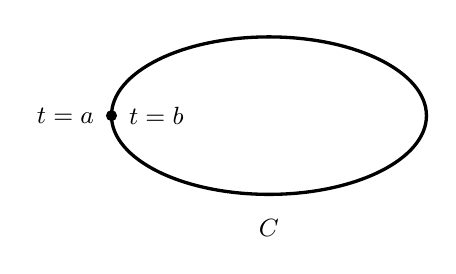
\begin{tikzpicture}
  \usetikzlibrary{arrows}
  \fill (-2,0) circle (2pt);
  \draw [black,line width=1.2pt] (-2,0) arc (180:90:2 and 1) node {\large $\blacktriangleright$};
  \draw [black,line width=1.2pt] (0,1) arc (90:-90:2 and 1) node {\large $\blacktriangleleft$};
  \draw [black,line width=1.2pt] (0,-1) arc (-90:-180:2 and 1);
  \node [below] at (0,-1.2) {\small $C$};
  \node [left] at (-2.1,0) {\small $t=a$};
  \node [right] at (-1.9,0) {\small $t=b$};
 \end{tikzpicture}}
 \qquad\qquad
 \subfloat[][Not closed]{
 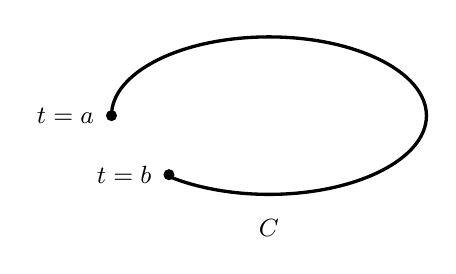
\begin{tikzpicture}
  \usetikzlibrary{arrows}
  \fill (-2,0) circle (2pt);
  \fill (-1.27,-0.75) circle (2pt);
  \draw [black,line width=1.2pt] (-2,0) arc (180:90:2 and 1) node {\large $\blacktriangleright$};
  \draw [black,line width=1.2pt] (0,1) arc (90:-90:2 and 1) node {\large $\blacktriangleleft$};
  \draw [black,line width=1.2pt] (0,-1) arc (-90:-130:2 and 1);
  \node [below] at (0,-1.2) {\small $C$};
  \node [left] at (-2.1,0) {\small $t=a$};
  \node [left] at (-1.37,-0.75) {\small $t=b$};
 \end{tikzpicture}}
 \caption[]{\quad Closed vs nonclosed curves}
 \label{fig:closedcurve}
\end{figure}
  

  If $\caminho$ is a closed curve, then line integrals over $\caminho$ are denoted by
  \begin{equation*}
    \doint_\caminho \funvect{f} \bp \dif \ell.
  \end{equation*}

  \begin{corollary}\label{clyLintGrad}
    If $\caminho \subseteq \bbR^n$ is a closed curve, and $\varphi:\caminho \to \bbR$ is $C^1$,  then
    \begin{equation*}
      \doint_\caminho \grad \varphi \bp \dif \ell = 0.
    \end{equation*}
  \end{corollary}

  \begin{definition}
    Let $U \subseteq \bbR^n$, and $\funvect{f}:U \to \bbR^n$ be a vector function.
    We say $\funvect{f}$ is a \negrito{conservative force} (or \negrito{conservative vector field}) if
    \begin{equation*}
      \doint \funvect{f} \bp \dif \ell = 0,
    \end{equation*}
    for all closed curves $\caminho$ which are completely contained inside $U$.
  \end{definition}

  Clearly if $\funvect{f} = - \grad \phi$ for some $C^1$ function $V:U \to \bbR$, then $\funvect{f}$ is conservative.
  The converse is also true provided $U$ is \negrito{simply connected}, which we'll return to later.
For conservative vector field:
  
\begin{align*}
  \dint_\gamma \vector F  \bp \dif \ell 
  &= \dint_\gamma \nabla \phi  \bp \dif \ell \\
  &= [\phi]_a^b\\
  &= \phi(b) - \phi(a)
\end{align*}  
  
We note that the result is \emph{independent of the path} $\caminho$ joining $a$ to $b$. 
\begin{center}
\begin{tikzpicture}[scale=1.8]
\begin{scope}[decoration={
    markings,
    mark=at position 0.5 with {\arrow{>}}}
    ] 
    \draw[postaction = {decorate}]  plot [smooth, tension=.4] coordinates {(0,0) (0.3,0.5) (1,0.6) (1.4,0.8) (1.5,1.1) (1.6,1.15)};
\end{scope}	
\draw[dashed,draw=Maroon] plot[smooth,tension=2] coordinates{(0,0) (-.1,0.3) (.2,.8) (0,1.1)  (.5,1.2) (.8,0.9) (1.4,1.1) (1.6,1.15)};
\fill (1.6,1.15) circle (1.5pt) node [right] {$B$};
\fill (0,0) circle (1.5pt) node[right]{$A$};
\node at (.7,.4) {$\gamma_1$};
\node at (.8,1.3) {$\gamma_2$};
\end{tikzpicture}
	
\end{center}

  
  
  
  
  \begin{exa} \label{not-simply-connected}
    If $\varphi$ fails to be $C^1$ even at one point, the above can fail quite badly.
    Let $\varphi(x, y) = \tan\inv(y/x)$, extended to $\bbR^2 - \set{(x, y) \st x \leq 0 }$ in the usual way.
    Then
    \begin{equation*}
      \grad \varphi = \dfrac{1}{x^2 + y^2} \colvec{ -y \\ x }
    \end{equation*}
    which is defined on $\bbR^2 - (0, 0)$.
    In particular, if $\caminho = \set{ (x, y) \st x^2 + y^2 = 1}$, then $\grad \varphi$ is defined on all of $\caminho$.
    However, you can easily compute
    \begin{equation*}
      \doint_\caminho \grad \varphi \bp \dif \ell = 2 \pi \neq 0.
    \end{equation*}
    The reason this doesn't contradict the previous corollary is that Corollary~\ref{clyLintGrad} requires $\varphi$ itself to be defined on all of $\caminho$, and not just $\grad \varphi$!
    This example leads into something called the \negrito{winding number} which we will return to later.
  \end{exa}

%   \todoin{Visualising conservative Fields}
  %%http://math.oregonstate.edu/BridgeBook/book/math/visconserv
 

\section{Test for a Gradient Field}

If a vector field $\vector{F}$ is a gradient field, and the potential $\varphi$ has continuous
second derivatives, then the second-order mixed partial derivatives
must be equal: 

\[\partiald{j}{F_i}{x} = \partiald{i}{F_j}{x} \text{for all } i,j\]

So if $\vector{F} = (F_1, \dots, F_n)$ is a gradient field and the
components of $\vector{F}$ have continuous partial derivatives, then we must have
\[\partiald{j}{f_i}{x} = \partiald{i}{f_j}{x} \text{for all } i,j\]
If these partial derivatives do not agree, then the vector
field cannot be a gradient field. 

This gives us an easy way to
determine that a vector field is \emph{not} a gradient field.

\begin{exa}
The vector field $(-y,x,-yx)$ is not a
  gradient field because {$M_y=-1$} is not equal to {$N_x=1$}.
\end{exa}



When $\vector{F}$ is defined on simple connected domain and has continuous partial derivatives, the check
works the other way as well.  

If $\vector{F} = (F_1, \dots, F_n)$ is  field and the
components of $\vector{F}$ have continuous partial derivatives, satisfying 
\[\partiald{j}{f_i}{x} = \partiald{i}{f_j}{x} \text{for all } i,j\] 
then $\vector{F}$ is a gradient field (i.e.,
there is a potential function $f$ such that $\vector{F} = \nabla f$).  This
gives us a very nice way of checking if a vector field is a gradient
field.  


\begin{exa}
The vector field $\vector{F}=(x,z,y)$ is
  a gradient field because $\vector{F}$ is defined on all of
  $\mathbb{R}^3$, each component has continuous partial derivatives,
  and $M_y=0=N_x$, $M_z=0=P_x$, and $N_z=1=P_y$.  Notice that
  $f=x^2/2+yz$ gives $\nabla f = \langle x,z,y\rangle=\vector{F}$.
\end{exa}
% 
% \begin{definition}[Exact differential forms]
% A \negrito{differential form} is an
% expression of the form {$Mdx+Ndy+Pdz$}.  On the other hand, if we have
% a function $f(x,y,z)$, the differential of $f$ is 
% $$df = Df d\vec x
% = \begin{bmatrix}f_x&f_y&f_z
% \end{bmatrix}\begin{bmatrix}dx\\dy\\dz\end{bmatrix}=f_x dx+f_y dy+f_z
% dz.$$ If a differential form is actually the differential of a
% function {$f$}, then the differential form is said to be
% \negrito{exact}.  The function {$f$} is called a \negrito{potential} for the
% differential form.  Notice that {$Mdx+Ndy+Pdz$} is exact if and only
% if {$\vector{F} = \langle M,N,P\rangle$} is a gradient field.
% \end{definition}
% 
% \begin{exa}
% The differential form $-ydx+xdy-yxdz$ is not
%   exact since the field $\langle-y,x,-yx\rangle$ is not a gradient
%   field (see above).  The differential form $xdx+zdy+ydz$ is exact
%   since the field $\langle x,z,y\rangle$ is a gradient field (see
%   above).
% \end{exa}
%  
%   
\subsection{Irrotational Vector Fields}

In this section we restrict our attention to  three dimensional space .

\begin{df}

Let  \(\vector{f}: U \to \mathbb{R}^3\) be a \(C^1\)
vector field defined in the open set  \(U\).
Then the vector \(\vector{f}\) is called
\negrito{irrotational} if and only if its curl
is \(\vector{0}\) everywhere in \(U\), i.e., if

\[\nabla \times \vector{f} \equiv \vector{0}.\]
 
\end{df}

For any \(C^2\) scalar field \(\varphi\) on \(U\),
we have
\[\nabla \times (\nabla \varphi) \equiv \vector{0}.\]
so every \(C^1\) conservative vector field on \(U\) is also an
irrotational vector field on \(U\).


Provided that \(U\) is simply connected, the
converse of this is also true: 

\begin{thm} Let \(U \subset \bbR^3\) be a simply connected domain and let $f$ be a $C^1$ vector field in $U$. 
Then are equivalents 
\begin{itemize}
 \item $f$ is a irrotational vector field;
 \item $f$ is a conservative vector field on \(U\)
\end{itemize}



\end{thm}

The proof of this theorem is presented in the Section \ref{conservative-potencial}.

The above statement is \emph{not} true in general if \(U\) is not simply
connected as we have already seen in the example \ref{not-simply-connected}.



  
  
\section{Conservative Fields}





\begin{df}
 A force field $F$, defined everywhere
in space (or within a simply-connected domain), is called
a \negrito{conservative force} or
conservative vector field if the curl of $\funvect{f}$ is zero: $\nabla \times \funvect{f} = \vector{0}.$
\end{df}




As a particle moves through a force field along a path $\caminho$, the
work done by the force is given by the  line integral
\[W = \dint_\caminho \funvect{f} \bp d\vector{r}\]

By the parametrization invariance this value is independent of how the particle travels along the path. 
And for a conservative force field, it is also independent of the path itself, and depends only on the starting and
ending points.
We observe also that if the field is conservative, the
work done can be more easily evaluated by realizing that a conservative
vector field can be written as the gradient of some scalar potential
function:
\[\funvect{f} = \nabla \phi\]

The work done is then simply the difference in the value of this
potential in the starting and end points of the path. If these points
are given by x = a and x = b, respectively:

\[W = \phi(b) - \phi(a)\]

The function $\phi$ is called the potential energy.

Therefore, if the starting and ending points are the
same, the work is zero for a conservative field:

\[\doint_\caminho \funvect{f} \bp d\vector{r} = 0\] 



% Now, we have  that the work done by a
% force is equal to the change in kinetic energy of the particle, but 
% mathematically, for a conservative force, the work done is minus the
% change in a function $\phi$ which we call the potential energy. As a
% consequence of these two, we arrive at the proposition that if only
% conservative forces act, the kinetic energy T plus the potential energy
% $\phi$ remains constant: 
% \begin{equation}
%  T+\phi=\text{constant} \label{eq:conservenergy}
% \end{equation}
% 
% 
% If we let $\phi_i$ denote the
% potential energy at the starting point and $\phi_i$ the potential energy at the final point, then, as the kinetic energy is given by $T=\dfrac{1}{2}mv$, the equation \ref{eq:conservenergy} can be written  as
% \[\dfrac{1}{2}mv_f+\phi_f= \dfrac{1}{2}mv_i+\phi_i.\]
% 
% 

  \subsection{Work and potential energy}
\begin{df}[Work and potential energy]
  If $\vector{F}(\vector{r})$ is a force, then $\dint_C \vector{F}\bp \d \ell$ is the \emph{work done} by the force along the curve $C$. It is the limit of a sum of terms $\vector{F}(\vector{r})\bp \delta \vector{r}$, ie. the force along the direction of $\delta \vector{r}$.
\end{df}

Consider a point particle moving under $\vector{F}(\vector{r})$ according to Newton's second law: $\vector{F}(\vector{r}) = m\ddot{\vector{r}}$.

Since the kinetic energy is defined as
\[
  T(t) = \dfrac{1}{2}m\dot{\vector{r}}^2,
\]
the rate of change of energy is
\[
  \dfrac{\d}{\d t}T(t) = m\dot{\vector{r}}\bp \ddot{\vector{r}} = \vector{F}\bp \dot{\vector{r}}.
\]
Suppose the path of particle is a curve $C$ from $\vector{a} = \vector{r}(\alpha)$ to $\vector{b} = \vector{r}(\beta)$, Then
\[
  T(\beta) - T(\alpha) = \dint_\alpha^\beta \dfrac{\d T}{\d t} \;\d t = \dint_\alpha^\beta \vector{F}\bp \dot{\vector{r}}\;\d t = \dint_C \vector{F}\bp \d \ell.
\]
So the work done on the particle is the change in kinetic energy.

\begin{df}[Potential energy]
  Given a conservative force $\vector{F} = -\nabla V$, $V(\vector{x})$ is the \emph{potential energy}. Then
  \[
    \dint_C \vector{F}\bp \d \ell = V(\vector{a}) - V(\vector{b}).
  \]
\end{df}
Therefore, for a conservative force, we have $\vector{F} = \nabla V$, where $V(\vector{r})$ is the potential energy.

So the work done (gain in kinetic energy) is the loss in potential energy. So the total energy $T + V$ is conserved, ie. constant during motion.

We see that energy is conserved for conservative forces. In fact, the converse is true --- the energy is conserved only for conservative forces.

 \section{The Second  Fundamental Theorem}



The gradient theorem states that if the vector field $\funvect{f}$ is the gradient of some scalar-valued function, then $\funvect{f}$ is a path-independent vector field. This theorem has a powerful converse:

\begin{thm}
 Suppose $U \subseteq \bbR^n$ is a domain of $\bbR^n$.
If $\funvect{f}$ is a path-independent vector field in $U$, then $\funvect{f}$ is the gradient of some scalar-valued function.
\end{thm} 


It is straightforward to show that a vector field is path-independent if and only if the integral of the vector field over every closed loop in its domain is zero. Thus the converse can alternatively be stated as follows: If the integral of $\funvect{f}$ over every closed loop in the domain of $\funvect{f}$ is zero, then $\funvect{f}$ is the gradient of some scalar-valued function.

\begin{proof}
 
 Suppose $U$ is an open, path-connected subset of $\bbR^n$, and $\vector{F} : U \to \bbR^n$ is a continuous
 and path-independent vector field. Fix some point   $\vector{a}$ of $U$, and define $f : U \to \bbR$ by

\[f(\vector{x}) := \dint_{\gamma[\vector{a}, \vector{x}]} \vector{F}(\vector{u}) \bp d\vector{u} \]
Here $\gamma[\vector{a}, \vector{x}]$ is any  differentiable curve in $U$ originating at $\vector{a}$ and terminating at $\vector{x}$. We know that $f$ is well-defined because $\funvect{f}$ is path-independent.

Let $\vector{v}$ be any nonzero vector in $\bbR^n$. By the definition of the directional derivative,

\begin{align} 
\dfrac{\partial f}{\partial \vector{v}}(\vector{x}) &= \lim_{t \to 0} \dfrac{f(\vector{x} + t\vector{v}) - f(\vector{x})}{t} \\
&= \lim_{t \to 0} \dfrac{\dint_{\gamma[\vector{a}, \vector{x} + t\vector{v}]} \vector{F}(\vector{u}) \bp d\vector{u} - \dint_{\gamma[\vector{a}, \vector{x}]} \vector{F}(\vector{u}) \bp d\vector{u}}{t} \\
&= \lim_{t \to 0} \dfrac{1}{t} \dint_{\gamma[\vector{x}, \vector{x} + t\vector{v}]} \vector{F}(\vector{u}) \bp d\vector{u}
\end{align}

To calculate the integral within the final limit, we must parametrize $\gamma[\vector{x}, \vector{x}+t\vector{v}]$. Since $\funvect{f}$ is path-independent, $U$ is open, and $t$ is approaching zero, we may assume that this path is a straight line, and parametrize it as 
$\vector{u}(s) = \vector{x} + s\vector{v}$ for $0 < s < t$. Now, since $\vector{u} '(s) = \vector{v}$, the limit becomes

\[ \lim_{t \to 0} \dfrac{1}{t} \dint_0^t \vector{F}(\vector{u}(s)) \bp \vector{u}'(s)\,\ds =  \dfrac{d}{dt} \dint_0^t \vector{F}(\vector{x} + s\vector{v}) \bp \vector{v}\,\ds \bigg|_{t=0} = \vector{F}(\vector{x}) \bp \vector{v} \]

Thus we have a formula for $\partial_\vector{v} f$, where $\vector{v}$ is arbitrary.. Let $\vector{x} = (x_1, x_2, \dots, x_n)$ 

\[\nabla f(\vector{x}) = \bigg( \dfrac{\partial f(\vector{x})}{\partial x_1}, \dfrac{\partial f(\vector{x})}{\partial x_2}, . . . , \dfrac{\partial f(\vector{x})}{\partial x_n} \bigg)  = \vector{F}(\vector{x})\]

Thus we have found a scalar-valued function $f$ whose gradient is the path-independent vector field $\funvect{f}$, as desired.
 
\end{proof}

\section{Constructing Potentials Functions}

If $\funvect{f}$  is a conservative field on an open connected set $U$, the line
integral of $\funvect{f}$ is independent of the path in $U$. Therefore we can find a potential  simply by
integrating $\funvect{f}$ from some fixed point $\vector{a}$ to an arbitrary point $\vector{x}$ in $U$, using any piecewise
smooth path lying in $U$. The scalar field so obtained depends on the choice of the initial
point $ a$. If we start from another initial point, say b, we obtain a new potential.
But, because of the additive property of line integrals,  and  can differ only by a constant,
this constant being the integral of $\funvect{f}$ from $\vector{a}$ to $\vector{b}$.

\todoin{ write Constructing Potentials Functions}

\paragraph{Construction of a potential on an open rectangle.}

If $\funvect{f}$ is a conservative vector field
on an open rectangle in $\bbR^n$, a potential $f$ can be constructed by integrating from a fixed
point to an arbitrary point along a set of line segments parallel to the coordinate axes.

\begin{figure}[h]
 \centering
 
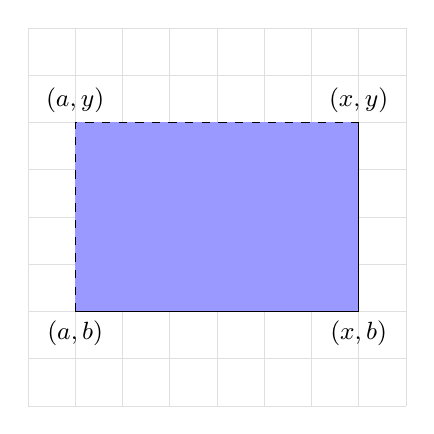
\begin{tikzpicture}[scale=0.6]
\draw[step=1cm,lightgray!50,very thin] (-2,-2) grid (6,6);
\fill[fill=blue!40!white] (-1,0) rectangle (5,4); 
\draw (-1,0)--(5,0)--(5,4);
\draw[dashed] (-1,0)--(-1,4)--(5,4);
   \node [below] at (-1,0) {\small $(a,b)$};
      \node [below] at (5,0) {\small $(x,b)$};
      \node [above] at (-1,4) {\small $(a,y)$};
       \node [above] at (5,4) {\small $(x,y)$};
\end{tikzpicture}
\end{figure}

We will simplify the deduction, assuming that $n=2$. In this case we can integrate first from (a, b) to
(x, b) along a horizontal segment, then from (x, b) to (x,y) along a vertical segment.
Along the horizontal segment we use the parametric representation
\[\gamma(t)=t\vector{i} + b\vector{j}, a<,t<,x,\]
and along the vertical segment we use the parametrization
\[\gamma_2(t) = x\vector{i} + t\vector{j}, b<t<y.\]
If $F(x,y) = F_1(x,y)\vector{i} + F_2(x,y)\vector{j}$, the resulting formula for a potential $f(x, y)$ is
\[ f(x, y) = \dint_a^b F_1(t, b) \dt + \dint_b^y F_2(x, t) \dt.\]
We could also integrate first from $(a, b)$ to $(a, y)$ along a vertical segment and then from
$(a, y)$ to $(x, y)$ along a horizontal segment as indicated by the dotted lines in Figure.
This gives us another formula for f(x, y),
\[f(x, y) = \dint_b^y F_2(a, t) \dt + \dint_a^x  F_2(t, y) \dt.\]
Both formulas  give the same value for $f(x, y)$ because the line integral
of a gradient is independent of the path.
 
 
\paragraph{Construction of a potential using anti-derivatives}

 But there's another way to find a potential of a conservative vector field: you use the fact that $\dfrac{\partial V}{\partial x} = F_x$ to conclude that $V(x,y)$ must be of the form $\dint_a^x F_x(u,y) du + G(y)$, and similarly $\dfrac{\partial V}{\partial y} = F_y$ implies that $V(x,y)$ must be of the form $\dint_b^y F_y(x,v) du + H(x)$.  So you find functions $G(y)$ and $H(x)$ such that $\dint_a^x F_x(u,y) du + G(y) = \dint_b^y F_y(x,v) du + H(x)$

 
\begin{exa}
  Show that 

\[\vector{F}=(e^x \cos y+yz)\vector{i}+(xz-e^x\sin y)\vector{j}+(xy+z)\vector{k}\]

is conservative over its natural domain and find a potential function for it.

\end{exa}


\begin{solu}
 


The natural domain of F is all of space, which is connected and simply connected. Let's define the following:

\[M=e^x\cos y+yz\]
\[N=xz-e^x\sin y\]
\[P=xy+z\]

and calculate
\[\dfrac{\partial P }{\partial x}=y=\dfrac{\partial M}{\partial z}\]
\[\dfrac{\partial P }{\partial y}=x=\dfrac{\partial N}{\partial z}\]
\[\dfrac{\partial N }{\partial x}=-e^x\sin y=\dfrac{\partial M}{\partial y}\]
Because the partial derivatives are continuous, F is conservative. Now that we know there exists a function f where the gradient is equal to F, let's find f.

\[\dfrac{\partial f }{\partial x}=e^x\cos y+yz\]
\[\dfrac{\partial f }{\partial y}=xz-e^x\sin y\]
\[\dfrac{\partial f }{\partial z}=xy+z\]

If we integrate the first of the three equations with respect to x, we find that 

\[f(x,y,z)=\dint(e^x\cos y+yz)dx=e^x\cos y+xyz+g(y,z)\]

where g(y,z) is a constant dependant on y and z variables. We then calculate the partial derivative with respect to y from this equation and match it with the equation of above. 

\[\dfrac{\partial }{\partial y}(f(x,y,z))=-e^x\sin y+xz+\dfrac{\partial g}{\partial y}=xz-e^x\sin y\]

This means that the partial derivative of g with respect to y is 0, thus eliminating y from g entirely and leaving at as a function of z alone. 
\[f(x,y,z)=e^x\cos y+xyz+h(z)\]

We then repeat the process with the partial derivative with respect to z.
\[\dfrac{\partial }{\partial z}(f(x,y,z))=xy+\dfrac{\mathrm{d} h}{\mathrm{d} z}=xy+z\]

which means that 
\[\dfrac{\mathrm{d} h}{\mathrm{d} z}= z\]

so we can find h(z) by integrating:
\[h(z)=\dfrac{z^2}{2}+C\]

Therefore,

\[f(x,y,z)=e^x\cos y+xyz+\dfrac{z^2}{2}+C\]

We still have infinitely many potential functions for F, one at each value of $C$.
\end{solu}
 
 \section{Green's Theorem in the Plane}
  
  \begin{df}
A \negrito{positively oriented curve} is a planar simple closed curve such that when travelling on it one always has the curve interior to the left. If in the previous  definition one interchanges left and right, one obtains a \negrito{negatively oriented curve}.
  \end{df}

\begin{figure}[h]
 \centering
 \subfloat[][positively oriented curve]{
 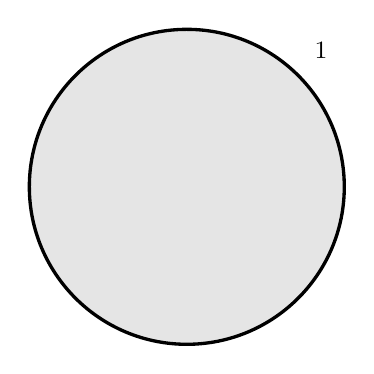
\begin{tikzpicture}
  \usetikzlibrary{arrows}
  \filldraw [black,line width=1.2pt,fill=black!10] (0:0) circle (2);
  %\filldraw [black,line width=1.2pt,fill=white] (0:0) circle (0.5);
  \node [above right] at (1.5,1.5) {\small $\ssub{\caminho}{1}$};
  %\node [above] at (0,0.5) {\small $\ssub{\caminho}{2}$};
%   \node at (0,1.35) {\small $\ssub{R}{1}$};
  %\node at (0,-1.35) {\small $\ssub{R}{2}$};
  %\node [rotate=45] at (-0.3536,0.3536) {\Large $\blacktriangleright$};
  %\node [rotate=45] at (0.3536,-0.3536) {\Large $\blacktriangleleft$};
  \node [rotate=-45] at (1.4142,1.4142) {\Large $\blacktriangleleft$};
   \node [rotate=-45] at (-1.4142,-1.4142) {\Large $\blacktriangleright$};
%   \draw [dashed] (0.5,0) -- (2,0);
%   \draw [dashed] (-0.5,0) -- (-2,0);
%   \draw [-latex] (1.05,0.15) -- (1.45,0.15);
%   \draw [latex-] (1.05,-0.15) -- (1.45,-0.15);
%   \draw [-latex] (-1.45,0.15) -- (-1.05,0.15);
%   \draw [latex-] (-1.45,-0.15) -- (-1.05,-0.15);
 \end{tikzpicture}}
 \qquad\qquad
 \subfloat[][positively oriented curve]{
 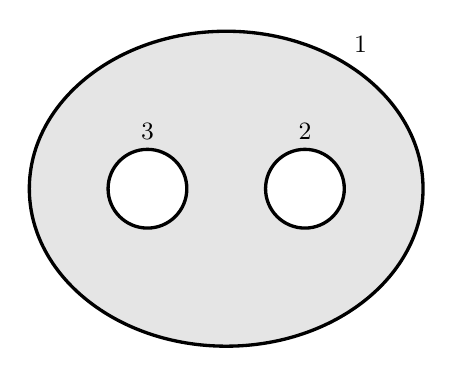
\begin{tikzpicture}
  \usetikzlibrary{arrows}
  \filldraw [black,line width=1.2pt,fill=black!10] (0,0) ellipse (2.5 and 2);
  \filldraw [black,line width=1.2pt,fill=white] (-1,0) circle (0.5);
  \filldraw [black,line width=1.2pt,fill=white] (1,0) circle (0.5);
  \node [above right] at (1.5,1.6) {\small $\ssub{\caminho}{1}$};
  \node [above] at (1,0.5) {\small $\ssub{\caminho}{2}$};
  \node [above] at (-1,0.5) {\small $\ssub{\caminho}{3}$};
%   \node at (0,1.35) {\small $\ssub{R}{1}$};
%   \node at (0,-1.35) {\small $\ssub{R}{2}$};
   \node [rotate=45] at (-1.3536,0.3536) {\Large $\blacktriangleright$};
   \node [rotate=45] at (0.6464,0.3536) {\Large $\blacktriangleright$};
   \node [rotate=45] at (-0.6464,-0.3536) {\Large $\blacktriangleleft$};
   \node [rotate=45] at (1.3536,-0.3536) {\Large $\blacktriangleleft$};
   \node [rotate=-31] at (1.5,1.6) {\Large $\blacktriangleleft$};
   \node [rotate=-31] at (-1.5,-1.6) {\Large $\blacktriangleright$};
%   \draw [dashed] (2.5,0) -- (1.5,0);
%   \draw [dashed] (0.5,0) -- (-0.5,0);
%   \draw [dashed] (-1.5,0) -- (-2.5,0);
%   \draw [-latex] (1.8,0.15) -- (2.2,0.15);
%   \draw [latex-] (1.8,-0.15) -- (2.2,-0.15);
%   \draw [-latex] (-0.2,0.15) -- (0.2,0.15);
%   \draw [latex-] (-0.2,-0.15) -- (0.2,-0.15);
%   \draw [-latex] (-2.2,0.15) -- (-1.8,0.15);
%   \draw [latex-] (-2.2,-0.15) -- (-1.8,-0.15);
 \end{tikzpicture}}
 \qquad\qquad
 \subfloat[][negatively oriented curve]{
 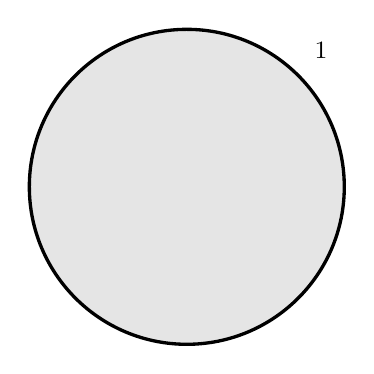
\begin{tikzpicture}
  \usetikzlibrary{arrows}
  \filldraw [black,line width=1.2pt,fill=black!10] (0:0) circle (2 and 2);
  %\filldraw [black,line width=1.2pt,fill=white] (0:0) circle (0.5);
  \node [above right] at (1.5,1.5) {\small $\ssub{\caminho}{1}$};
  %\node [above] at (0,0.5) {\small $\ssub{\caminho}{2}$};
%   \node at (0,1.35) {\small $\ssub{R}{1}$};
  %\node at (0,-1.35) {\small $\ssub{R}{2}$};
  %\node [rotate=45] at (-0.3536,0.3536) {\Large $\blacktriangleright$};
  %\node [rotate=45] at (0.3536,-0.3536) {\Large $\blacktriangleleft$};
  \node [rotate=135] at (1.4142,1.4142) {\Large $\blacktriangleleft$};
   \node [rotate=135] at (-1.4142,-1.4142) {\Large $\blacktriangleright$};
%   \draw [dashed] (0.5,0) -- (2,0);
%   \draw [dashed] (-0.5,0) -- (-2,0);
%   \draw [-latex] (1.05,0.15) -- (1.45,0.15);
%   \draw [latex-] (1.05,-0.15) -- (1.45,-0.15);
%   \draw [-latex] (-1.45,0.15) -- (-1.05,0.15);
%   \draw [latex-] (-1.45,-0.15) -- (-1.05,-0.15);
 \end{tikzpicture}}
 \qquad\qquad
 \caption[]{\quad Orientations of Curves}
 \label{fig:multconn}
\end{figure}  

We will now see a way of evaluating the line integral of a \emph{smooth} vector field
around a simple closed curve. 
A vector field $\vector{f}(x,y) = P(x,y)\,\vector{i} + Q(x,y)\,\vector{j}$ is \textbf{smooth} if its
component functions $P(x,y)$ and $Q(x,y)$ are smooth.\index{vector field!smooth}
We will use
\emph{Green's Theorem} (sometimes called \emph{Green's Theorem in the plane}) to relate the \emph{line} integral around
a closed curve with a \emph{double} integral over the region inside the curve:\index{Green's Theorem}


  \begin{theorem}[Green's Theorem - Simple Version]\label{thmGreens-simple}
  Let $\Omega$ be a region in $\bbR^2$ whose boundary is a simple closed curve $\caminho$ which is piecewise smooth.
  Let $\vector{f}(x,y) = P(x,y)\,\vector{i} + Q(x,y)\,\vector{j}$ be a smooth vector field defined on both
  $\Omega$ and $\caminho$. Then
  \begin{equation}\label{eqn:green}
   \olineintvec{\caminho}{f}{r} ~=~ \iint\limits_{\Omega} \left( \frac{\partial Q}{\partial x} - \frac{\partial P}{\partial y} \right)
   \,dA ~,
  \end{equation}
  where $\caminho$ is traversed so that $\Omega$ is always on the left side of $\caminho$.
\end{theorem}
\begin{proof}
 We will prove the theorem in the case for a \emph{simple} region $\Omega$, that is, where the boundary curve $\caminho$ can be
 written as $C = \ssub{\caminho}1 \cup \ssub{\caminho}{2}$ in two distinct ways:
 \begin{align}
  \ssub{\caminho}{1} &= \text{the curve $y = \ssub{y}{1}(x)$ from the point $\ssub{X}{1}$ to the point $\ssub{X}{2}$}\\
  \ssub{\caminho}{2} &= \text{the curve $y = \ssub{y}{2}(x)$ from the point $\ssub{X}{2}$ to the point $\ssub{X}{1}$,}
 \end{align}
 where $\ssub{X}{1}$ and $\ssub{X}{2}$ are the points on $C$ farthest to the left and right, respectively; and
 \begin{align}
  \ssub{\caminho}{1} &= \text{the curve $x = \ssub{x}{1}(y)$ from the point $\ssub{Y}{2}$ to the point $\ssub{Y}{1}$}\\
  \ssub{\caminho}{2} &= \text{the curve $x = \ssub{x}{2}(y)$ from the point $\ssub{Y}{1}$ to the point $\ssub{Y}{2}$,}
 \end{align}
 where $\ssub{Y}{1}$ and $\ssub{Y}{2}$ are the lowest and highest points, respectively, on $\caminho$.
 See Figure 
 \piccaption[]{}\parpic(\textwidth,0in){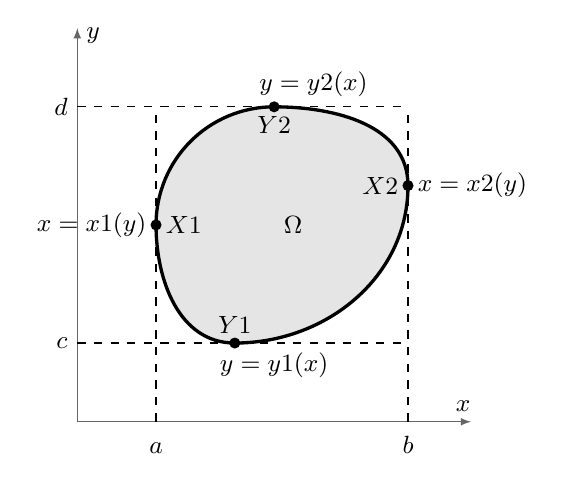
\begin{tikzpicture}
  \usetikzlibrary{arrows}
  \draw [black!60,line width=0.3pt,-latex,anchor=base] (0,0) -- (5,0)
    node[black,shift={(0,-0.4)}] at (1,0) {\small $a$}
    node[black,shift={(0,-0.4)}] at (4.2,0) {\small $b$};
  \draw [black!60,line width=0.3pt,-latex] (0,0) -- (0,5);
  \pgfputat{\pgfpointxyz{4.9}{0.2}{0}}{\pgfbox[center,center]{\small $x$}}
  \pgfputat{\pgfpointxyz{0.2}{4.9}{0}}{\pgfbox[center,center]{\small $y$}}
  \filldraw [black,line width=1.2pt,fill=black!10] (1,2.5) to[out=90,in=180] node [sloped]
  {\large $\blacktriangleleft$} (2.5,4) to[out=0,in=90] (4.2,3) to[out=270,in=0] node [sloped]
  {\large $\blacktriangleright$}(2,1) to[out=180,in=270] (1,2.5);
  \node [above] at (3,4) {\small $y = \ssub{y}{2}(x)$};
  \node [below] at (2.5,1) {\small $y = \ssub{y}{1}(x)$};
  \node [right] at (4.2,3) {\small $x = \ssub{x}{2}(y)$};
  \node [left] at (1,2.5) {\small $x = \ssub{x}{1}(y)$};
  \node [below] at (2.5,4) {\small $\ssub{Y}{2}$};
  \node [above] at (2,1) {\small $\ssub{Y}{1}$};
  \node [left] at (4.2,3) {\small $\ssub{X}{2}$};
  \node [right] at (1,2.5) {\small $\ssub{X}{1}$};
  \node [right] at (2.5,2.5) {\small $\Omega$};
  \node [left] at (4,1.5) {\small $\caminho$};
  \draw [dashed] (1,0) -- (1,4);
  \draw [dashed] (4.2,0) -- (4.2,4);
  \draw [dashed] (0,4) -- (4.2,4);
  \draw [dashed] (0,1) -- (4.2,1);
  \node [left] at (0,4) {\small $d$};
  \node [left] at (0,1) {\small $c$};
  \fill (1,2.5) circle (2pt);
  \fill (2.5,4) circle (2pt);
  \fill (4.2,3) circle (2pt);
  \fill (2,1) circle (2pt);
 \end{tikzpicture}\piccaptioninside}
 \par\mbox{}\newline\vspace{2mm}\picskip{0}

 \par\noindent Integrate $P(x,y)$ around $\caminho$ using the representation $\caminho = \ssub{\caminho}{1} \cup \ssub{\caminho}{2}$
\noindent Since $y = \ssub{y}{1}(x)$ along $\ssub{\caminho}{1}$ (as $x$ goes from $a$ to $b$) and $y = \ssub{y}{2}(x)$ along
 $\ssub{\caminho}{2}$ (as $x$ goes from $b$ to $a$), as we see from Figure, then we have
 \begin{align*}
  \oint_\caminho P(x,y)\,dx ~&=~ \int_{\ssub{\caminho}{1}} P(x,y)\,dx ~+~ \int_{\ssub{\caminho}{2}} P(x,y)\,dx\\
   &=~ \int_a^b P(x,\ssub{y}{1}(x))\,dx ~+~ \int_b^a P(x,\ssub{y}{2}(x))\,dx\\
   &=~ \int_a^b P(x,\ssub{y}{1}(x))\,dx ~-~ \int_a^b P(x,\ssub{y}{2}(x))\,dx\\[6pt]
   &=~ -\int_a^b \left( P(x,\ssub{y}{2}(x)) ~-~ P(x,\ssub{y}{1}(x)) \right)\,dx\\[6pt]
   &=~ -\int_a^b \left( P(x,y) \,\Big|_{y = \ssub{y}{1}(x)}^{y = \ssub{y}{2}(x)} \,\right)\,dx\\[6pt]
   &=~ -\int_a^b \int_{\ssub{y}{1}(x)}^{\ssub{y}{2}(x)} \frac{\partial P(x,y)}{\partial y}\,dy\,dx ~~\text{(by the
    Fundamental Theorem of Calculus)}\\[6pt]
   &=~ -\iint\limits_{\Omega} \frac{\partial P}{\partial y}\,dA ~.
 \end{align*}
 Likewise, integrate $Q(x,y)$ around $\caminho$ using the representation $\caminho = \ssub{\caminho}{1} \cup \ssub{\caminho}{2}$.
 Since $x = \ssub{x}{1}(y)$ along $\ssub{\caminho}{1}$ (as $y$ goes from $d$ to $c$) and $x = \ssub{x}{2}(y)$ along
 $\ssub{\caminho}{2}$ (as $y$ goes from $c$ to $d$), as we see from Figure , then we have
 \begin{align*}
  \oint_\caminho Q(x,y)\,dy ~&=~ \int_{\ssub{\caminho}{1}} Q(x,y)\,dy ~+~ \int_{\ssub{\caminho}{2}} Q(x,y)\,dy\\
   &=~ \int_d^c Q(\ssub{x}{1}(y),y)\,dy ~+~ \int_c^d Q(\ssub{x}{2}(y),y)\,dy\\
   &=~ -\int_c^d Q(\ssub{x}{1}(y),y)\,dy ~+~ \int_c^d Q(\ssub{x}{2}(y),y)\,dy\\[6pt]
   &=~ \int_c^d \left( Q(\ssub{x}{2}(y),y) ~-~ Q(\ssub{x}{1}(y),y) \right)\,dy\\[6pt]
   &=~ \int_c^d \left( Q(x,y) \,\Big|_{x = \ssub{x}{1}(y)}^{x = \ssub{x}{2}(y)} \,\right)\,dy\\[6pt]
   &=~ \int_c^d \int_{\ssub{x}{1}(y)}^{\ssub{x}{2}(y)} \frac{\partial Q(x,y)}{\partial x}\,dx\,dy ~~\text{(by the
    Fundamental Theorem of Calculus)}\\[6pt]
   &=~ \iint\limits_{\Omega} \frac{\partial Q}{\partial x}\,dA ~,~\text{and so}
 \end{align*}

 \begin{align*}
  \olineintvec{\caminho}{f}{r} ~&=~ \oint_\caminho P(x,y)\,dx + \oint_\caminho Q(x,y)\,dy\\[6pt]
   &=~ -\iint\limits_{\Omega} \frac{\partial P}{\partial y}\,dA + \iint\limits_{\Omega} \frac{\partial Q}{\partial x}\,dA\\[6pt]
   &=~ \iint\limits_{\Omega} \left( \frac{\partial Q}{\partial x} - \frac{\partial P}{\partial y} \right)\,dA ~.
 \end{align*}
\end{proof}
  

The Green Theorem can be generalized:
  
  \begin{theorem}[Green's Theorem]\label{thmGreens}
    Let $\Omega \subseteq \bbR^2$ be a bounded domain whose exterior boundary is a piecewise $C^1$ curve $\caminho$.
    If $\Omega$ has holes, let $\caminho_1$, \dots, $\caminho_N$ be the interior boundaries.
    If $\funvect{f}:\bar \Omega  \to \bbR^2$ is $C^1$, then
    \begin{equation*}
      \dint_\Omega \left[\partial_1 F_2 - \partial_2 F_1\right] \, dA
	= \doint_{\caminho} \funvect{f} \bp \dif \ell + \sum_{i = 1}^N \doint_{\caminho_i} \funvect{f} \bp \dif \ell,
    \end{equation*}
    where all line integrals above are computed by traversing the exterior boundary \negrito{counter clockwise}, and every interior boundary \negrito{clockwise}.
  \end{theorem}
  \begin{remark}
    A common convention is to denote the \negrito{boundary} of $\Omega$ by $\partial \Omega$ and write
    \begin{equation*}
      \partial \Omega = \caminho \cup \left[ \bigcup_{i = 1}^N \caminho_i \right].
    \end{equation*}
    Then Theorem~\ref{thmGreens} becomes
    \begin{equation*}
      \dint_\Omega \left[\partial_1 F_2 - \partial_2 F_1\right] \, dA
	= \doint_{\partial \Omega} \funvect{f} \bp \dif \ell,
    \end{equation*}
    where again the exterior boundary is oriented \negrito{counter clockwise} and the interior boundaries are all oriented \negrito{clockwise}.
  \end{remark}
  \begin{remark}
    In the differential form notation, Green's theorem is stated as
    \begin{equation*}
      \dint_\Omega \left[ \partial_x Q - \partial_y P \right] \, dA
      = \dint_{\partial \Omega} P \, \dx + Q \, \dy,
    \end{equation*}
    $P, Q:\bar \Omega \to \bbR$ are $C^1$ functions.
    (We use the same assumptions as before on the domain $\Omega$, and orientations of the line integrals on the boundary.)
  \end{remark}
  \begin{remark}
    Note, Green's theorem requires that $\Omega$ is bounded and $\funvect{f}$ (or $P$ and $Q$) is $C^1$ on \emph{all} of $\Omega$.
    If this fails at even one point, Green's theorem need not apply anymore!
  \end{remark}



  
  \begin{proof}
    The full proof is a little cumbersome.     But the main idea can be seen by first proving it when $\Omega$ is a 
square.
%, and then applying a coordinate transformation.
    Indeed, suppose first $\Omega = (0, 1)^2$.
    \begin{center}
 
\begin{tikzpicture} [x=2cm,y=2cm, >=triangle 45]  
% axes
  \draw [->, >=angle 45] (-.2,0) -- (1.2,0) node [right] {$x$};
  \draw [->, >=angle 45] (0,-.2) -- (0,1.2) node [right] {$y$};
% square 
  \draw [line width=1.5, addarrow=.125, addarrow=.375, addarrow=.628, 
         addarrow=.875] (.2,.2) -- ++(.9,0) -- ++(0,.9) -- ++(-.9,0) --cycle;
% ticks
  \draw (.2,1pt)  -- +(0,-2pt) node[anchor=north] {$a$};
  \draw (1.1,1pt) -- +(0,-2pt) node[anchor=north] {$b$};
  \draw (1pt,.2)  -- +(-2pt,0) node[anchor=east] {$c$};
  \draw (1pt,1.1) -- +(-2pt,0) node[anchor=east] {$d$};
\end{tikzpicture}  

\end{center}
 
    Then the fundamental theorem of calculus gives
    \begin{equation*}
      \dint_\Omega \left[ \partial_1 F_2 - \partial_2 F_1 \right] \, dA
	= \dint_{y = 0}^1 \left[ F_2(1, y) - F_2(0, y) \right] \, \dy
	  - \dint_{x = 0}^1 \left[ F_1(x, 1) - F_1(x, 0) \right] \, \dx
    \end{equation*}
    The first integral is the line integral of $\funvect{f}$ on the two vertical sides of the square, and the second one is line integral of $\funvect{f}$ on the two horizontal sides of the square.
    This proves Theorem~\ref{thmGreens} in the case when $\Omega$ is a square.

 For line integrals, when adding two rectangles with a common edge the common 
edges are traversed in opposite directions so the sum is just the line integral
over the outside boundary. 
\begin{center}


\begin{tikzpicture} [ x=2.5cm,y=2.5cm, >=triangle 45]  
% Produced by hand
% two squares
  \draw [line width=1.5, addarrow=.125, addarrow=.375, addarrow=.628, 
         addarrow=.875] (0,0) -- ++(.5,0) -- ++(0,.5) -- ++(-.5,0) --cycle;
  \begin{scope} [shift={($(0,.5) +(0,1ex)$)}]
     \draw [line width=1.5, addarrow=.125, addarrow=.375, addarrow=.628, 
            addarrow=.875] (0,0) -- ++(.5,0) -- ++(0,.5) -- ++(-.5,0) --cycle;
  \end{scope}
% big rectangle
  \begin{scope} [shift={($(.5,.5) +(2ex,0)$)}]
     \node at (0,0) [right=2ex] {\Huge $=$};
  \end{scope}
  \begin{scope} [shift={($(1,0) +(4ex,0)$)}]
     \draw [line width=1.5, addarrow=.125, addarrow=.375, addarrow=.628, 
            addarrow=.875] (0,0) -- ++(.5,0) -- ++(0,1) -- ++(-.5,0) --cycle;
  \end{scope}
\end{tikzpicture}
 
\end{center}


Similarly when adding a lot of rectangles: 
everything cancels except the outside boundary. This extends Green's Theorem
on a rectangle to Green's Theorem on a sum of rectangles.  Since any region can
be approximated as closely as we want by a sum of rectangles, Green's Theorem
must hold on arbitrary regions.
   
    
    
%     Now let $U$ be an arbitrary region for which there exists a $C^2$ coordinate transformation $\varphi:\Omega \to U$, where $\Omega$ is the unit square.
%     We assume that $\varphi$ also maps $\partial \Omega$ to $\partial U$ and \emph{preserves the orientation of the boundaries}.
%     (One can show that this will imply $\det D\varphi > 0$ in $U$.)
%     Now, using Green's theorem on the square,
%     \begin{equation*}
%       \doint_{\partial U} \funvect{f} \bp \dif \ell
% 	= \doint_{\partial \Omega} (D \varphi)^T \funvect{f} \circ \varphi \bp \dif \ell
% 	= \dint_\Omega (\partial_1 G_2 - \partial_2 G_1) \, dA,
%     \end{equation*}
%     where
%     \begin{equation*}
%       G = (D \varphi)^T \funvect{f} \circ \varphi = \sum_{i,j} \partial_i \varphi_j F_j \circ \varphi \, e_i
%     \end{equation*}
% 
%     Now we compute using the chain rule
%     \begin{equation*}
% 	\partial_1 G_2 - \partial_2 G_1
% 	  = \sum_{i, j} \partial_2 \varphi_j \, \partial_i F_j\bigr|_\varphi \, \partial_1 \varphi_i
% 	    - \partial_1 \varphi_j \, \partial_i F_j\bigr|_\varphi \, \partial_2 \varphi_i
% 	  = \paren[\big]{ \partial_1 F_2 - \partial_2 F_1 }\circ \varphi \, \det(D \varphi).
%     \end{equation*}
%     Thus, by the change of variable theorem,
%     \begin{equation*}
%       \dint_\Omega \paren[\big]{\partial_1 G_2 - \partial_2 G_1} \, dA
% 	= \dint_\Omega \paren[\big]{ \partial_1 F_2 - \partial_2 F_1 }\circ \varphi \, \det(D \varphi) \, dA
% 	= \dint_U \paren[\big]{ \partial_1 F_2 - \partial_2 F_1} \, dA,
%     \end{equation*}
%     finishing the proof.
  \end{proof}

  

\begin{center}

\begin{tikzpicture} [line width = 1.6]  
% Produced by hand
  \draw [step=.25, gray, very thin] (-.2,-2.2) grid (3.2,1.2);
  \coordinate (A) at (0,0);
  \coordinate (B) at (.3,-1);
  \coordinate (C) at (1,-1.6);
  \coordinate (D) at (2,-1.8);
  \coordinate (E) at (2.7,-1);
  \coordinate (F) at (3,0);
  \coordinate (G) at (2,1);
  \coordinate (H) at (1,.5);
    \draw [addarrow=.25, addarrow=.8, >=triangle 45]
                (A) to [out=270, in=130] 
                (B) to [out=310, in=160]
                (C) to [out=340, in=180]
                (D) to [out=0,   in=250]
                (E) to [out=70,  in=270]
                (F) to [out=90,  in=0]
                (G) to [out=180, in=0] 
                (H) to [out=180, in=90]
                (A);
  \begin{scope} [shift={($(3,-.5) +(2ex,0)$)}]
     \node at (0,0) [right=2ex] {\Huge $\approx$};
  \end{scope}
  \begin{scope} [shift={($(3,0)+(12ex,0)$)}, line width = 1, >=angle 45]  
    \draw [step=.25, gray, very thin] (-.2,-2.2) grid (3.2,1.2);
    %We can't define the coordinates outside the scopes because
    %then they aren't shifted --even when used inside a scope
    \coordinate (A) at (0,0);
    \coordinate (B) at (.3,-1);
    \coordinate (C) at (1,-1.6);
    \coordinate (D) at (2,-1.8);
    \coordinate (E) at (2.7,-1);
    \coordinate (F) at (3,0);
    \coordinate (G) at (2,1);
    \coordinate (H) at (1,.5);
    \draw [gray]
          (A) to [out=270, in=130] 
          (B) to [out=310, in=160]
          (C) to [out=340, in=180]
          (D) to [out=0,   in=250]
          (E) to [out=70,  in=270]
          (F) to [out=90,  in=0]
          (G) to [out=180, in=0] 
          (H) to [out=180, in=90]
          (A);
    \draw [line width=1.6, >=triangle 45, addarrow=.025, addarrow=.25, 
           addarrow=.6, addarrow=.925]
          (.25,0) -- (.25,-.75) -- (.5,-.75) -- (.5,-1.25) -- (1,-1.25)
          -- (1,-1.5) -- (1.5,-1.5) -- (1.5,-1.75) -- (2.25,-1.75)
          -- (2.25,-1.5) -- (2.5,-1.5) -- (2.5,-.75) -- (2.75,-.75)
          -- (2.75,.5) -- (2.5,.5) -- (2.5,.75) -- (1.75, .75)
          -- (1.75, .5) -- (1.25,.5) -- (1.25,.25) -- (.25,.25) -- cycle;
  \end{scope}
\end{tikzpicture}
\end{center}

  
  
%   
%   \begin{remark}
%     The above strategy will only work if the domain has no holes.
%     In the presence of holes, you can make one or more cuts and then find a coordinate transformation $\varphi:\Omega \to U$ as above.
%     The only difference is now part of the boundary of $\Omega$ will be mapped to the cut you just made.
%     The boundary integral over this piece, however, will cancel since it will now be traversed twice in opposite directions.
%   \end{remark}

\begin{exa}\label{exmp:greenexa}
  Evaluate $\doint_{C} (x^2 + y^2 )\,dx + 2xy\,\dy$, where $C$ is the boundary traversed counterclockwise of the region
  $R = \lbrace\,(x,y): 0 \le x \le 1,~2x^2 \le y \le 2x \,\rbrace$.\vspace{-1mm}
  \end{exa}

  \begin{center}
 
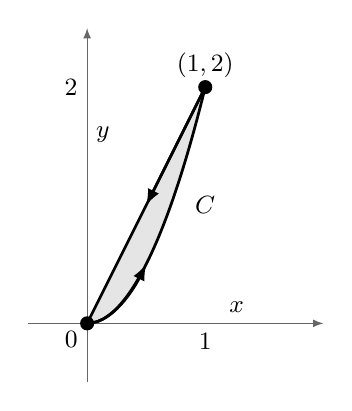
\begin{tikzpicture}[scale=1.5]
   \usetikzlibrary{arrows}
   \fill [fill=black!10] (0,0) parabola (1,2) -- (0,0);
   \draw [black!60,line width=0.3pt,-latex] (-0.5,0) -- (2,0);
   \draw [black!60,line width=0.3pt,-latex] (0,-0.5) -- (0,2.5);
   \pgfputat{\pgfpointxyz{1.9}{0.2}{0}}{\pgfbox[center,center]{\small $x$}}
   \pgfputat{\pgfpointxyz{0.2}{2.4}{0}}{\pgfbox[center,center]{\small $y$}}
   \pgfputat{\pgfpointxyz{-0.2}{-0.2}{0}}{\pgfbox[center,center]{\small $0$}}
   \draw [line width=1pt] (0,0) parabola (1,2);
   \draw [line width=1pt,-latex] (0,0) parabola (0.5,0.5);
   \draw [line width=1pt] (0,0) -- (1,2);
   \draw [line width=1pt,-latex] (1,2) -- (0.5,1);
   \node [right,above] at (1,2) {\small $(1,2)$};
   \node [left] at (0,2) {\small $2$};
   \node [below] at (1,0) {\small $1$};
   \node at (1,1) {\small $C$};
   \fill (0,0) circle (1.7pt);
   \fill (1,2) circle (1.7pt);
  \end{tikzpicture}  
  \end{center}


  \begin{solu}
   $R$ is the shaded region in Figure above. By Green's Theorem, for
 $P(x,y)=x^2 + y^2$ and $Q(x,y)=2xy$, we have
 \begin{align*}
  \doint_C (x^2 + y^2 )\,dx + 2xy\,\dy ~&=~ \iint\limits_{\Omega} \left( \dfrac{\partial Q}{\partial x} -
   \dfrac{\partial P}{\partial y} \right)\,dA\\
   &=~ \iint\limits_{\Omega} (2y - 2y)\,dA
   ~=~ \iint\limits_{\Omega} 0\,dA ~=~ 0 ~.
 \end{align*}
 There is another way to see that the answer is zero. The vector field
 $\vector{f}(x,y) = ( x^2 + y^2 )\,\vector{i} + 2xy\,\vector{j}$ has a potential function
 $F(x,y)=\dfrac{1}{3}x^3 + xy^2$, and so $\olineintvec{C}{f}{r} = 0$.
   \end{solu}

\begin{exa}\label{exmp:greenhole}
 Let $\vector{f}(x,y) = P(x,y)\,\vector{i} + Q(x,y)\,\vector{j}$, where
 \begin{displaymath}
  P(x,y) = \dfrac{-y}{x^2 + y^2} \quad\text{and}\quad Q(x,y) = \dfrac{x}{x^2 + y^2} ~,
 \end{displaymath}
 and let $R =\lbrace\,(x,y): 0 < x^2 + y^2 \le 1\,\rbrace$. For the boundary curve $C:x^2 + y^2 = 1$, traversed
 counterclockwise, it was shown in Exercise 9(b) in Section 4.2 that $\olineintvec{C}{f}{r} = 2\pi$. But
 \begin{displaymath}
  \dfrac{\partial Q}{\partial x} ~=~ \dfrac{y^2 - x^2}{(x^2 + y^2 )^2} ~=~ \dfrac{\partial P}{\partial y} ~
  \Rightarrow ~
  \iint\limits_{\Omega} \left( \dfrac{\partial Q}{\partial x} - \dfrac{\partial P}{\partial y} \right)\,dA ~=~
  \iint\limits_{\Omega} 0 \,dA = 0~.
 \end{displaymath}
\end{exa}
This would seem to contradict Green's Theorem. However, note that $R$ is not the \emph{entire} region enclosed by $C$,
since the point $(0,0)$ is not contained in $R$. That is, $R$ has a ``hole'' at the origin, so Green's Theorem does not
apply.


\section{Application of Green's Theorem: Area}

Green's theorem can be used to compute area by line integral. 
Let $C$ be a positively oriented, piecewise smooth, simple closed curve in a plane, and let $U$ be the region bounded by $C$
The area of domain $U$ is given by $A = \diint_{U}dA$. 

Then if we choose $P$ and $M$ such that $\dfrac{\partial Q}{\partial x} - \dfrac{\partial P}{\partial y} = 1$, the area is given by
\[A = \doint_{C} (P\, \dx + Q\, \dy).\]

Possible formulas for the area of $U$ include:

\[A=\doint_{C} x\, \dy = -\doint_{C} y\, \dx = \dfrac{1}{2} \doint_{C} (-y\, \dx + x\, \dy).\]



  \begin{corollary} \label{greenarea}
    Let $\Omega \subseteq \bbR^2$ be  bounded set  with a $C^1$ boundary $\partial \Omega$, then
    \begin{equation*}
      \area{\Omega}
	= \dfrac{1}{2} \dint_{\partial \Omega} \left[ -y \, \dx + x \, \dy \right]
	= \dint_{\partial \Omega} -y \, \dx
	= \dint_{\partial \Omega} x \, \dy
    \end{equation*}
  \end{corollary}
  
  
\begin{exa}
 Use Green's Theorem to calculate the area of the disk $D$ of radius $r$.

\end{exa}


\begin{solu}
The boundary of $D$ is the circle of radius $r$:
\begin{align*}
  C(t) = (r\cos t, r\sin t), \quad 0 \le t \le 2\pi.
\end{align*}
Then
\begin{align*}
  C'(t) = (-r\sin t, r\cos t),
\end{align*}
and, by Corollary \ref{greenarea},
\begin{align*}
  \text{area of } D &= \iint dA\\
  &=  \frac{1}{2} \int_C x\,dy - y\,dx\\
  &= \frac{1}{2} \int_0^{2\pi} [(r\cos t)(r\cos t) - (r\sin t)(-r\sin t)]dt
  \\
  &=
  \frac{1}{2}  \int_0^{2\pi} r^2 (\sin^2t+\cos^2t) dt = \frac{r^2}{2}\int_0^{2\pi}
  dt
  = \pi r^2.
\end{align*}
  
\end{solu}
  
  

\begin{exa}
Use the  Green's theorem for computing the area of the region bounded by the x -axis and the arch of the cycloid:
\[    x=t-\sin(t), \quad y=1-\cos(t), \quad 0\leq t\leq 2\pi\]
\end{exa}

\begin{solu}
$$ \text{Area}(D) = \iint\limits_D dA =  \oint\limits_C-ydx. $$
Along the $x$-axis, you have $y = 0$, so you only need to compute the integral over the arch of the cycloid. Note that your parametrization of the arch is a clockwise parametrization, so in the following calculation, the answer will be the minus of the area:
$$\int_0^{2\pi} (\cos(t) - 1)(1 - \cos(t)) dt = - \int_0^{2\pi} 1 - 2\cos(t) + \cos^2(t) dt = -3\pi. $$
\end{solu}




  
  
  \begin{corollary}[Surveyor's Formula]
    Let $P \subseteq \bbR^2$ be a (not necessarily convex) polygon whose vertices, ordered counter clockwise,
    are $(x_1, y_1)$, \dots, $(x_N, y_N)$.
    Then
    $$
      \area{P} = \dfrac{(x_1 y_2 - x_2 y_1) + (x_2 y_3 - x_3 y_2) + \cdots + (x_N y_1 - x_1 y_N)}{2}.
    $$
  \end{corollary}
  
  \begin{proof}
   Let $P$ be the set of points belonging to the polygon. We have that \[A=\diint_{P} \dx \dy.\]
   
   Using the Corollary \ref{greenarea} we have  
   \[\diint_{P}dxdy=\int_{\partial P}\frac{x\,dy}{2}-\frac{y\,dx}{2}.\] 
   We can write $\partial  P=\bigcup_{i=1}^{n} L(i)$, where $L(i)$ is the line segment from $(x_i,y_i)$ to $(x_{i+1},y_{i+1})$. With this notation, we may write 
   \[\int_{\partial P}\frac{x\,dy}{2}-\frac{y\,dx}{2}=\sum_{i=1}^n\int_{A(i)}\frac{x\,dy}{2}-\frac{y\,dx}{2}=\frac{1}{2}\sum_{i=1}^n\int_{A(i)}{x\,dy}-{y\,dx}.\] 
   
   Parameterizing the line segment, we can write the integrals as
   \[\frac{1}{2}\sum_{i=1}^n\int_0^1{(x_i+(x_{i+1}-x_i)t)(y_{i+1}-y_i)}-{(y_i+(y_{i+1}-y_i)t)(x_{i+1}-x_i)\,dt}.\] Integrating  we get \[\frac{1}{2}\sum_{i=1}^n\frac{1}{2}[(x_i+x_{i+1})(y_{i+1}-y_i)- (y_{i}+y_{i+1})(x_{i+1}-x_i)].\] simplifying  yields the result
   \[\area{P}=\frac{1}{2}\sum_{i=1}^n(x_iy_{i+1}-x_{i+1}y_i).\]
  \end{proof}

  
 
\section{Vector forms of Green's Theorem}

\begin{theorem}[Stokes' Theorem in the Plane] Let 
$\vector{F}= L\vector{i} + M\vector{j}$. Then 

\[
  \oint_\caminho \vector{F}\cdot \d \ell =
  \int_\Omega\nabla \times \,\vector{F}\cdot \d \mathbf S
\]
\end{theorem}

\begin{proof}
\[
  \nabla \times \,\vector{F} = \left(\frac{\partial  M}{\partial  x} - \frac{\partial  L}{\partial  y}\right)\hat {k}
\]
Over the region $R$ we can write $\d x \,\d y = \d S$ and $\d \mathbf S = \hat {k}\,\d S$. Thus using Green's Theorem:
\begin{align*}
  \oint_\caminho \vector{F}\cdot \d \ell 
  &= \int_\Omega\hat {k}\cdot\nabla \times \vector{F}\, \d S\\
  &= \int_\Omega\nabla \times \,\vector{F}\cdot \d \mathbf S
\end{align*}
\end{proof}



\begin{theorem}[Divergence Theorem in the Plane]. Let $\vector{F}=  M\vector{i} - L\vector{j}$ Then 
\[
  \int_R\nabla \bp\vector{F}\,\d x\,\d y = \oint_\caminho\vector{F}\cdot \hat {n}\,\d s
\]
\end{theorem}


\begin{proof}
 

\[
  \nabla \bp\,\vector{F} = \frac{\partial M}{\partial x} - \frac{\partial L}{\partial y}
\]
and so Green's theorem can be rewritten as 
\[
  \int_\Omega\nabla \bp\,\vector{F}\,\d x\,\d y = \oint_\caminho F_1\,\d y - F_2\,\d x
\]
Now it can be shown that
\[
  \hat {n}\,\d s = (\d y \vector{i} -\d x \vector{j})
\]
here s is arclength along $C$, and $\hat {n}$ is the unit normal to $C$. Therefore we can rewrite
Green’s theorem as
\[
  \int_R\nabla \bp\vector{F}\,\d x\,\d y = \oint_\caminho\vector{F}\cdot \hat {n}\,\d s
\]


\end{proof}



\begin{theorem}[Green's identities in the Plane]
 Let $\phi(x,y)$ and $\psi(x,y)$ be two scalar functions  $\mathcal{C}^{2}$, defined in the open set $\Omega \subset \mathbb{R}^{2}$.
\[
  \oint_\caminho \phi \frac{\partial \psi}{\partial n}\,\d s
  = \int_\Omega \phi \nabla^2 \psi +  (\partial \phi)\cdot(\partial \psi)]\,\d x\,\d y
\]
and 
\[
  \oint_\caminho  \left[\phi\frac{\partial \psi}{\partial n}- \psi\frac{\partial \phi}{\partial n}\right]
  \,\d s
  = \int_\tau 
  (\phi \nabla^2\psi - \psi \nabla^2\phi)\,\d x\,\d y
\]
\end{theorem}


\begin{proof}
If we use the divergence theorem:
\[
  \int_S \nabla \bp\,\vector{F}\,\d x\,\d y
  = \oint_\caminho\vector{F}\cdot \hat  n \,\d s
\]
then we can calculate down the corresponding Green identities. These are 
\[
  \oint_\caminho \phi \frac{\partial \psi}{\partial n}\,\d s
  = \int_\Omega \phi \nabla^2 \psi +  (\partial \phi)\cdot(\partial \psi)]\,\d x\,\d y
\]
and 
\[
  \oint_\caminho  \left[\phi\frac{\partial \psi}{\partial n}- \psi\frac{\partial \phi}{\partial n}\right]
  \,\d s
  = \int_\tau 
  (\phi \nabla^2\psi - \psi \nabla^2\phi)\,\d x\,\d y
\]

\end{proof}
